\problemname{Minecraft Speedrunning}
\noindent

\illustration{.3}{mcsr.png}{A video clip from Harry's Minecraft-speedrunning.}

Harry and his friends have recently started playing Minecraft together, and are trying to complete the game as fast as possible.

Harry's gang has now managed to gather all the resources they need to reach \textit{The Stronghold}, the place one needs to reach before the game can end.

The positions between the gang's current position and the Stronghold's position can be modelled on a number line where Harry's gang is currently at position $0$, and the Stronghold is located at position $S$.

In Minecraft, there are two worlds: \textit{Overworld} and \textit{Nether}. Harry's gang and the Stronghold exist in the Overworld.
The Nether can also be modelled as a number line, but all coordinates are compressed with a factor $8$: 
a position $x$ in the Nether corresponds to the position $8x$ in the Overworld.

Along the number line in the Nether, there are $N$ destroyed \textit{Netherportals}. 
Portal $i$ is located at position $x_i$ in the Nether and leads to the position $8x_i$ in the Overworld.
To be able to use the portal $i$, it needs to first be repaired, which takes $t_i$ seconds. 
Note that the portal must be repaired regardless of whether one travels from the Overworld to the Nether or from the Nether to the Overworld.

Harry's gang can walk along the number line in the Overworld to a portal exit of their choice (position $8x_i$) or directly
to the Stronghold at position $S$. 
The walking speed is $1$, so it takes as much time to walk as the distance on the number line.

What is the minimum number of seconds it can take for Harry's gang to reach the Stronghold from position $0$ in the Overworld? 

\section*{Input}
The first line contains two integers $N$ and $S$ ($2 \le N \le 2 \cdot 10^5$), ($1 \le S \le 10^9$), the number of destroyed Nether portals and the position for the Stronghold in the Overworld.

Each of the following $N$ lines contain two integers $x_i$ and $t_i$ ($1 \le x_i \le 10^9$, $8x_i < S$), ($1 \le t_i \le 10^9$), the position for portal $i$ in the Nether and the time it takes to repair the portal (in seconds).

It is guaranteed that $x_i < x_{i+1}$ for all $1 \le i < N$.

\section*{Output}
Print one integer, the minimum number of seconds it can take for Harry's gang to reach the Stronghold from position $0$ in the Overworld. 


\section*{Scoring}
Your solution will be tested on a set of test groups, each worth a number of points. Each test group contains
a set of test cases. To get the points for a test group you need to solve all test cases in the test group.

\noindent
\begin{tabular}{| l | l | p{12cm} |}
  \hline
  \textbf{Group} & \textbf{Poitns} & \textbf{Constraints} \\ \hline
  $1$    & $15$        & $N = 2$ \\ \hline 
  $2$    & $19$        & $t_i = 1$ for all $i = 1, \dots, N$. \\ \hline 
  $3$    & $27$        & $N \le 1000$ \\ \hline
  $4$    & $39$        & No additional constraints. \\ \hline 
\end{tabular}

\section*{Explanation of Sample 3}

\begin{figure}[h]
  \centering
  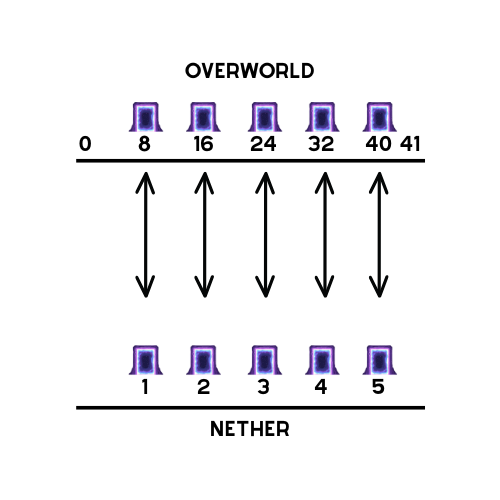
\includegraphics[width=0.6\linewidth]{fresh.png}
  \caption{Portals according to Sample 3.}
\end{figure}


We see that the fastest way to reach the Stronghold is to go:
\begin{itemize}
  \item from position $0$ to position $16$ by portal $2$, (takes $16$ seconds),
  \item repair portal $2$ and go through it to position $2$ in the Nether (takes $t_2 = 5$ seconds),
  \item then go to position $4$ in the Nether (takes $2$ seconds),
  \item repair portal $4$ and go through it (takes $t_4 = 5$ seconds),
  \item and finally go from position $32$ in the Overworld to the Stronghold by position $41$ (takes $9$ seconds).
\end{itemize}

In total, this takes $16 + 5 + 2 + 5 + 9 = 37$ seconds, which can be shown to be the least possible amount.

